\documentclass[11pt]{article}
\usepackage[utf8]{inputenc}
\usepackage[russian]{babel}
\usepackage[T1]{fontenc}
\usepackage{amssymb,amsmath,clrscode,graphicx,indentfirst,haskell}

\author{Олег Смирнов}
\title{Курс kiev-clrs -- Лекция 10. Красно-чёрные деревья}
\date{13 июня 2009 г.}

\begin{document}
\maketitle
\tableofcontents

\newpage
\setlength{\parskip}{1ex plus 0.5ex minus 0.2ex}
\section{Цель лекции}
\begin{itemize}
\item Красно-чёрные деревья поиска
\item Изометрия между RB и 2-3-4 деревьями
\end{itemize}

\section{Сбалансированные поисковые деревья}
Сбалансированным называется дерево, высота которого гарантировано не превышает $\lg n$ для $n$ элементов. Таким образом операции поиска, вставки и удаления на нём работают за $O(\lg n)$ итераций.

Существуют разные подходы к организации таких структур:
\begin{itemize}
\item AVL-деревья (придуманы в 1962 году в СССР)
\item 2-3 деревья
\item 2-3-4 деревья
\item AA-деревья
\item RB-деревья (Red-Black)
\item Списки с пропусками (Skip lists)
\item Декартовы деревья (Treaps = Tree + Heap)
\end{itemize}
2-3 и 2-3-4 являются разновидностями более общей структуры -- B-деревьев.
\section{Красно-чёрные деревья}
Красно-чёрным называется бинарное поисковое дерево, у которого каждому узлу сопоставлена дополнительный аттрибут -- цвет и для которого выполняются следующие свойства:
\begin{enumerate}
\item Каждый узел промаркирован красным или чёрным цветом
\item Корень и конечные узлы (листья) дерева -- чёрные
\item У красного узла родительский узел -- чёрный
\item Все простые пути из любого узла $x$ до листьев содержат одинаковое количество чёрных узлов -- black-height(x)
\item Чёрный узел может иметь чёрного родителя
\end{enumerate}
\begin{figure}[ht]
  \centering
  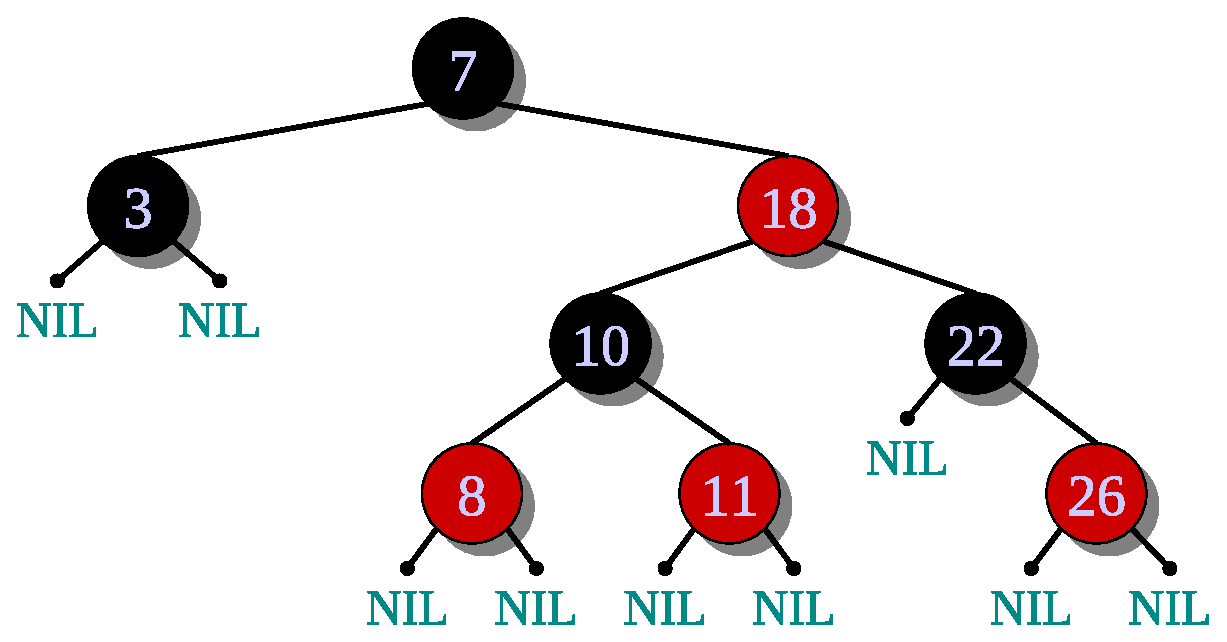
\includegraphics[width=3in]{lecture10/rbtree.eps}
  \caption{Пример красно-чёрного дерева}
  \label{fig:rbtree}
\end{figure}
При подсчете количества чёрных узлов считаем листья (конечные узлы) за единицу.
\begin{figure}[ht]
  \centering
  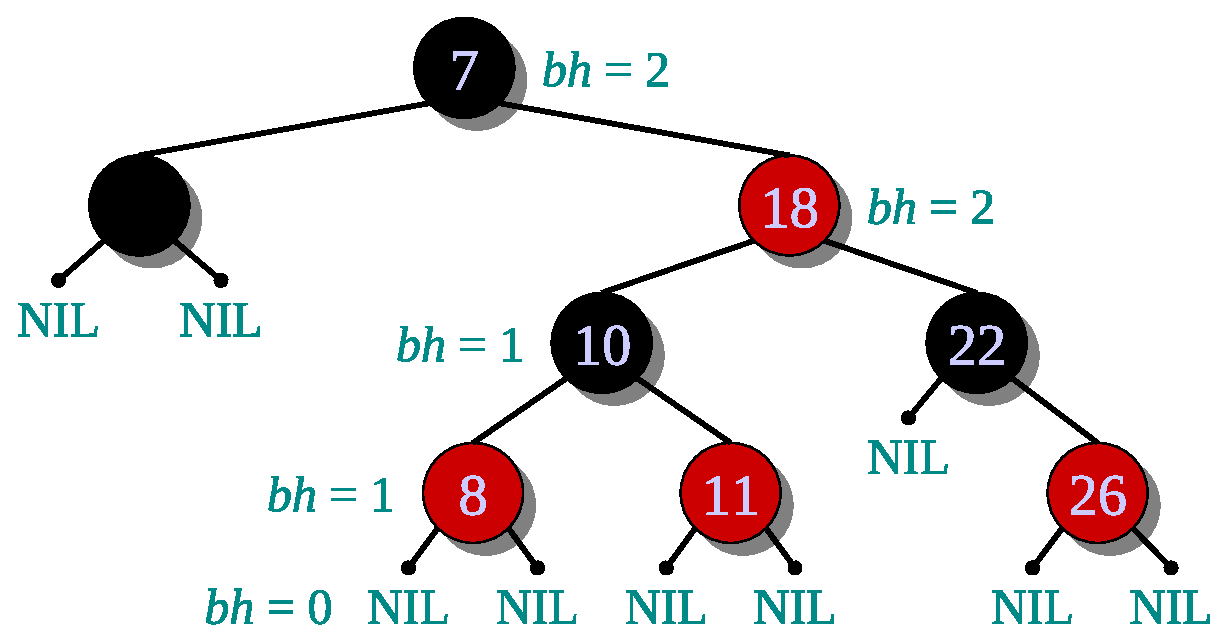
\includegraphics[width=3in]{lecture10/bh_rbtree.eps}
  \caption{Свойство black-height(x)}
  \label{fig:bh-rbtree}
\end{figure}
Свойства дерева (в основном третье и четвертое) гарантируют его логарифмическую высоту.

Сконструировать красно-чёрное дерево из входного массива довольно просто. Например, можно положить все узлы чёрными. Задача разработать алгоритм вставки (и удаления) элемента, который бы позволил поддерживать свойство балансировки и при этом работал за логарифмическое время.
\section{Высота красно-чёрного дерева}
Теорема: Красно-чёрное дерево с $n$ ключами имеет высоту
\begin{equation*}
  h \leqslant 2 \lg (n+1) = O(\lg n)
\end{equation*}
Схема доказательства:
\begin{enumerate}
\item Совмещаем все красные узлы с родительскими чёрными (они существуют по свойству 2) начиная с корня
\item В результате получим дерево, каждый узел котрого имеет 2, 3 или 4 потомка
\item В следствии свойства 4 красно-чёрного дерева, все листья 2-3-4 дерева будут иметь одинаковую глубину -- black-height корня исходного дерева
\item Пусть дерево из п.2 имеет высоту $h'$. Тогда $h' \geqslant h/2$, т.к. не более половины узлов на каждом пути -- красные
\begin{figure}[ht]
  \centering
  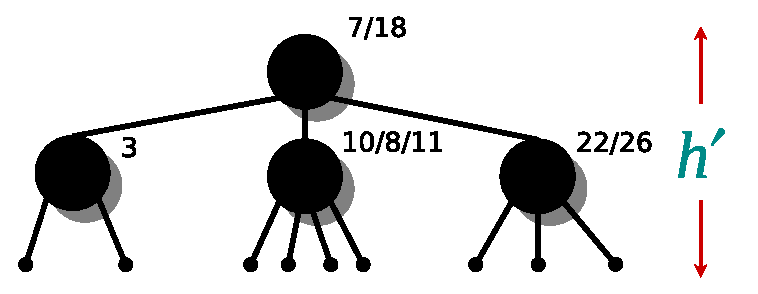
\includegraphics[width=3in]{lecture10/2-3-4.eps}
  \caption{2-3-4 дерево}
  \label{fig:2-3-4}
\end{figure}
\item Количество листьев не изменяется и равно $n+1$ для обоих деревьев, т.к. в красно-чёрном дереве все внутренние узлы имеют ровно два листа
\item В 2-3-4 дереве высоты $h'$ количество листьев $n+1$ ограничено: $2^{h'} \leqslant n+1 \leqslant 4^{h'}$
\item Тогда:
\begin{align*}
  n+1 \geqslant 2^{h'} \\
  \lg(n+1) \geqslant h' \geqslant h/2 \\
  h \leqslant 2 \lg (n+1)
\end{align*}
\end{enumerate}
%
\section{Алгоритмы на красно-чёрных деревьях}
\subsection{Поиск и запросы}
Алгоритм поиска Search, а также алгоритмы Min, Max, Successor и Predecessor аналогичны алгоритмам для бинарных поискых деревьев.
\subsection{Вставка и удаление}
В отличии от запросов, модификация может нарушить свойства красно-чёрных деревьев. Поэтому необходимы дополнительные операции:
\begin{itemize}
\item Вставка/удаление аналогично BST
\item Изменение цветов узлов
\item Реструктуризация связей между узлами с помощью ``вращений''
\end{itemize}
Вращения бывают ``правые'' и ``левые''. Операции вращения сохраняют свойства поискового дерева: $a \in \alpha, b \in \beta, c \in \gamma \Rightarrow a \leqslant A \leqslant b \leqslant B \leqslant c$ и выполняются за $O(1)$ итераций.
\begin{figure}[ht]
  \centering
  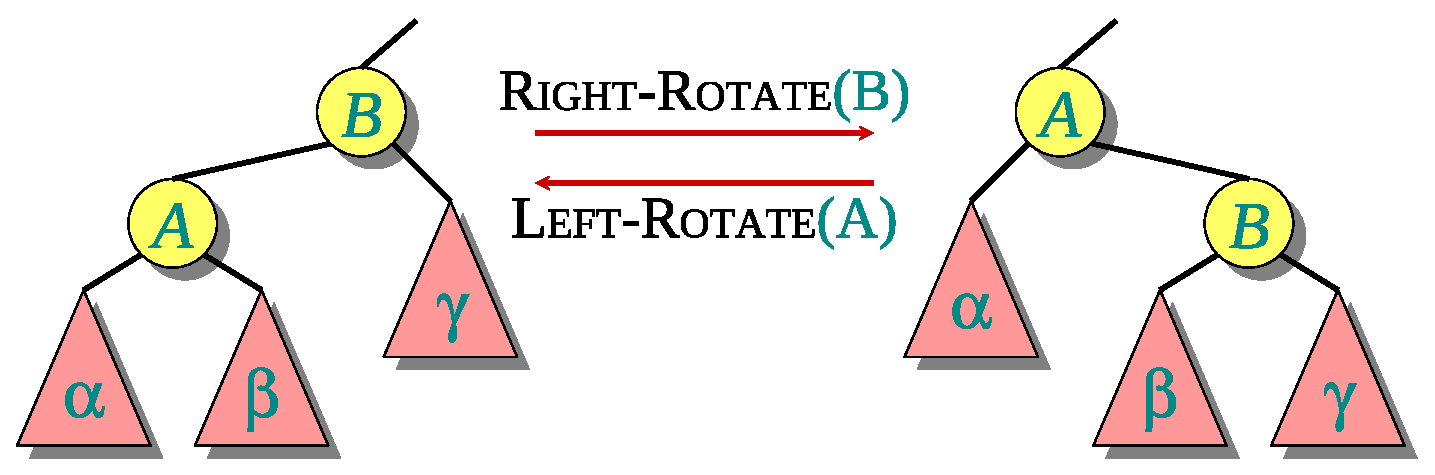
\includegraphics[width=4in]{lecture10/rotations.eps}
  \caption{Правое вращение B и левое вращение A}
  \label{fig:rotations}
\end{figure}
Идея алгоритма вставки:
\begin{itemize}
\item Добавить элемент $x$ помощью BST Tree\_Insert
\item Установить цвет $x$ -- красный
\item Если третье свойство ``красно-чёрности'' нарушено, ``передвигать'' нарушение вверх по дереву, выполняя операции изменения цвета и поворотов
\item Цвета должны изменяться таким образом, чтоб не нарушить четвертое свойство
\item В конце работы цвет корня дерева -- чёрный
\end{itemize}
На первом шаге (рис. \ref{fig:example1}) новый элемент (15) красного цвета. Нарушено третье свойство, т.к. его родитель (11) также красный. Если новый элемент сделать чёрным, то нарушится четвертое свойство, т.к. тогда из 11 левый путь будет содержать один чёрный элемент, а правый -- два.
\begin{figure}[h!]
  \centering
  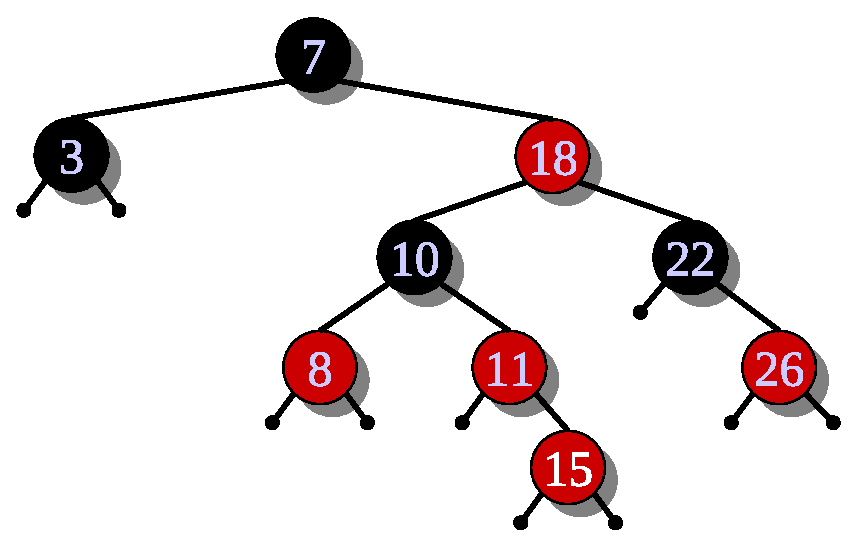
\includegraphics[width=3in]{lecture10/example1.eps}
  \caption{Пример, шаг 1: добавляем элемент $x=15$}
  \label{fig:example1}
\end{figure}

``Прародитель'' нового узла (10) чёрного цвета (рис. \ref{fig:example2}), а два его потомка -- красные. Это значит, что можно изменить цвета, сместив нарушение на уровень 10.
\begin{figure}[h!]
  \centering
  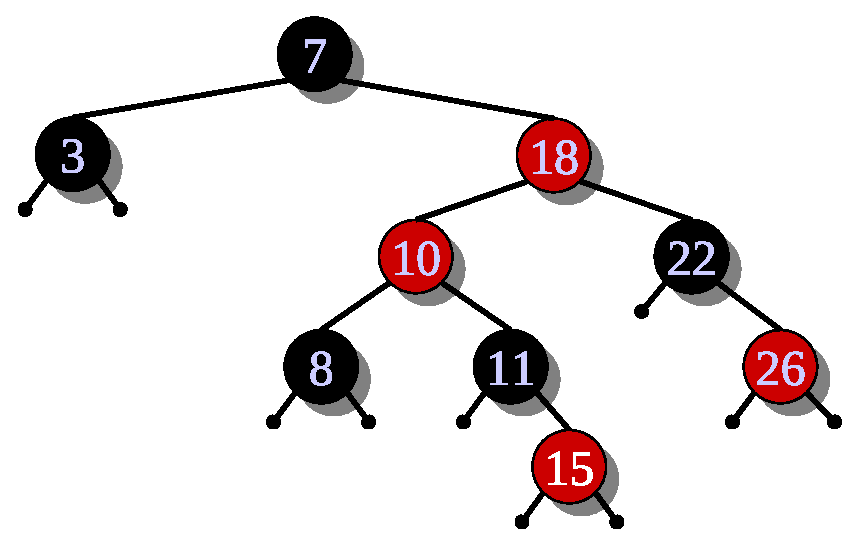
\includegraphics[width=3in]{lecture10/example2.eps}
  \caption{Пример, шаг 2: изменяем цвет 8, 10 и 11}
  \label{fig:example2}
\end{figure}

Изменить цвет элемента 7 и его потомков 3 и 18 нельзя, т.к. они разных цветов (рис. \ref{fig:example3}). Вместо этого выполняем правое вращение относительно элемента 18.
\begin{figure}[h!]
  \centering
  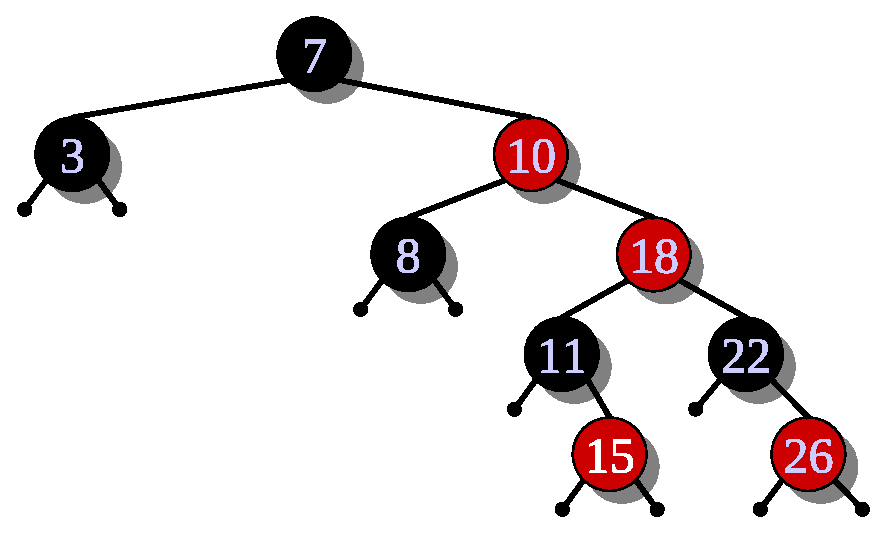
\includegraphics[width=3in]{lecture10/example3.eps}
  \caption{Пример, шаг 3: правое вращение относительно 18}
  \label{fig:example3}
\end{figure}

После вращение относительно 7, дерево снова становится сбалансированным (рис. \ref{fig:example4}). Изменяем цвет нового корня (10) на чёрный.
\begin{figure}[h!]
  \centering
  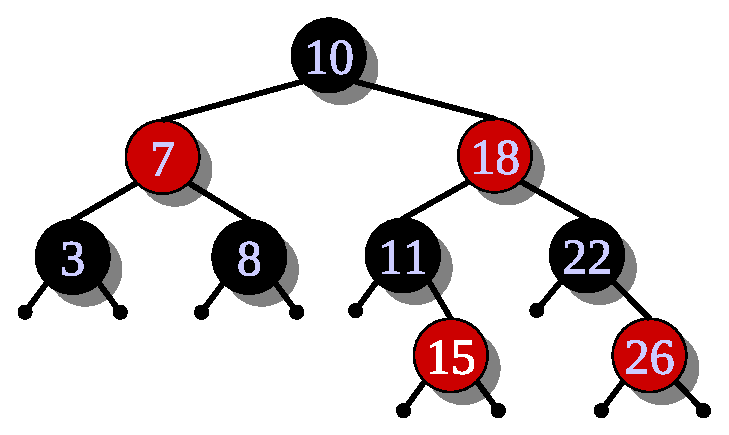
\includegraphics[width=2.5in]{lecture10/example4.eps}
  \caption{Пример, шаг 4: левое вращение относительно 7}
  \label{fig:example4}
\end{figure}

Алгоритм выполняет не более двух вращений и не более $\lg n$ шагов, пока не будет достигнут корень дерева.

Итак, алгоритм рассматривает три возможных случая:
\begin{itemize}
\item В случае 1, когда прародитель узла $x$ -- чёрный, а второй потомок прародителя (``дядя'') -- красный или в симметричном (когда потомки $A$ поменяны местами), чёрный цвет $C$ ``опускается'' на $A$ и $D$ (на родителя и ``дядю''), а прародитель $C$ становится красным. После этого нужно продолжить балансировку, т.к. родитель $C$ тоже может быть красным
\begin{figure}[h!]
  \centering
  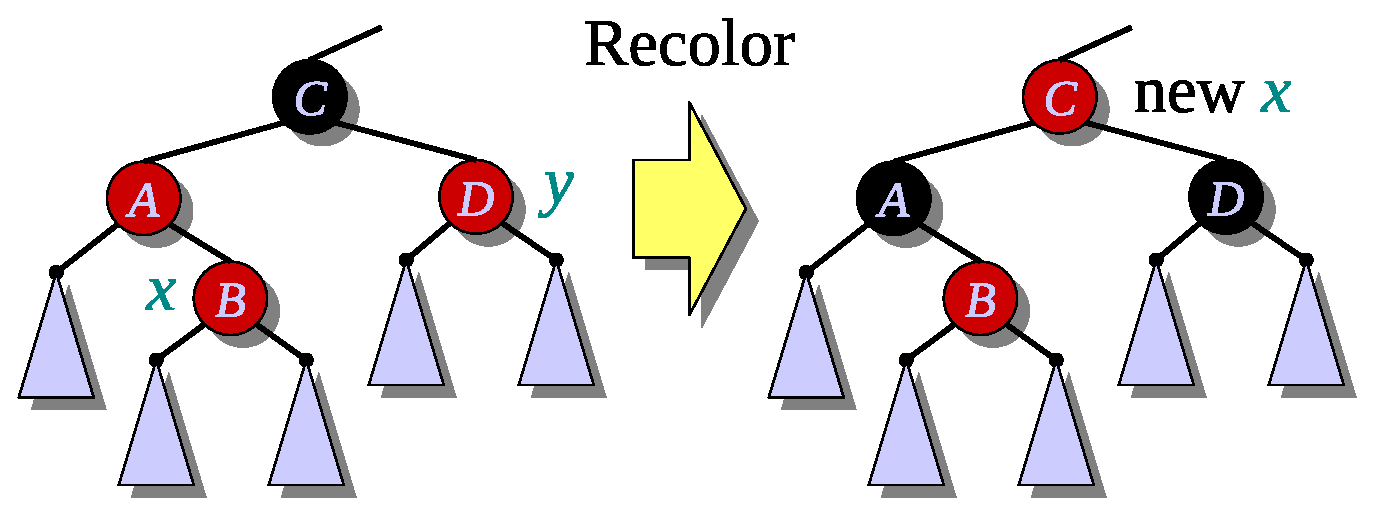
\includegraphics[width=4.5in]{lecture10/case1.eps}
  \caption{Случай 1}
  \label{fig:case1}
\end{figure}
\item В случае 2 ``дядя'' узла $x$ -- корень поддерева $y$ -- чёрный. Цвет менять нельзя, т.к. это нарушит четвертое свойство. Левое вращение относительно $A$ сводит ситуацию к случаю 3
\begin{figure}[h!]
  \centering
  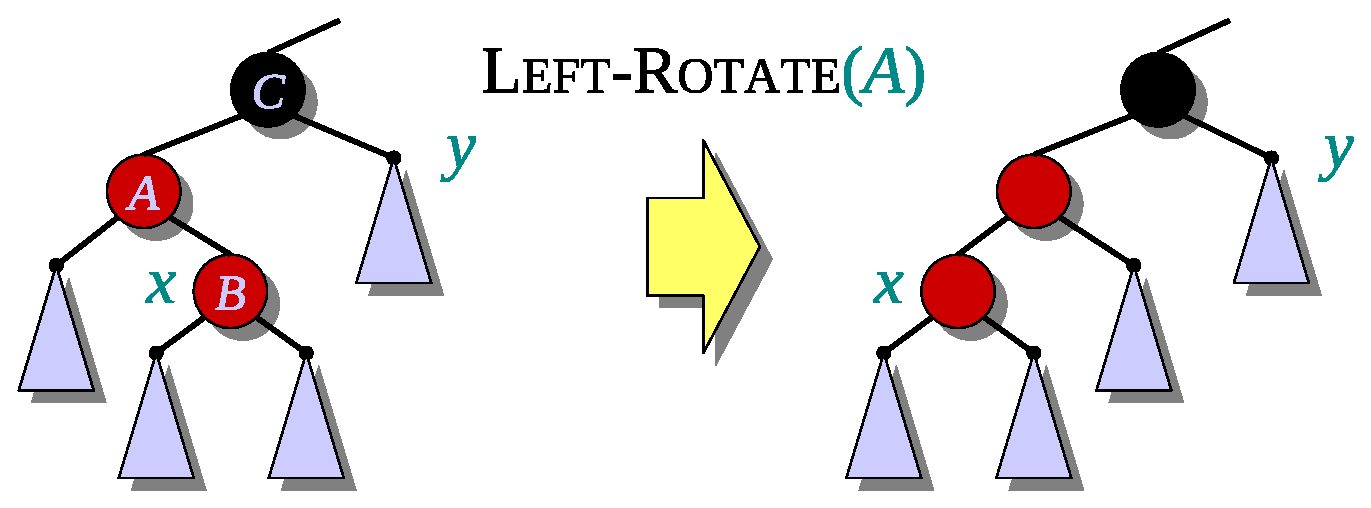
\includegraphics[width=4.5in]{lecture10/case2.eps}
  \caption{Случай 2}
  \label{fig:case2}
\end{figure}
\item В случае 3 правое вращение относительно элемента $B$ исправляет нарушения. Больше модификаций не требутся независимо от того, какой цвет у родителя $C$ ($B$ после вращения)
\begin{figure}[h!]
  \centering
  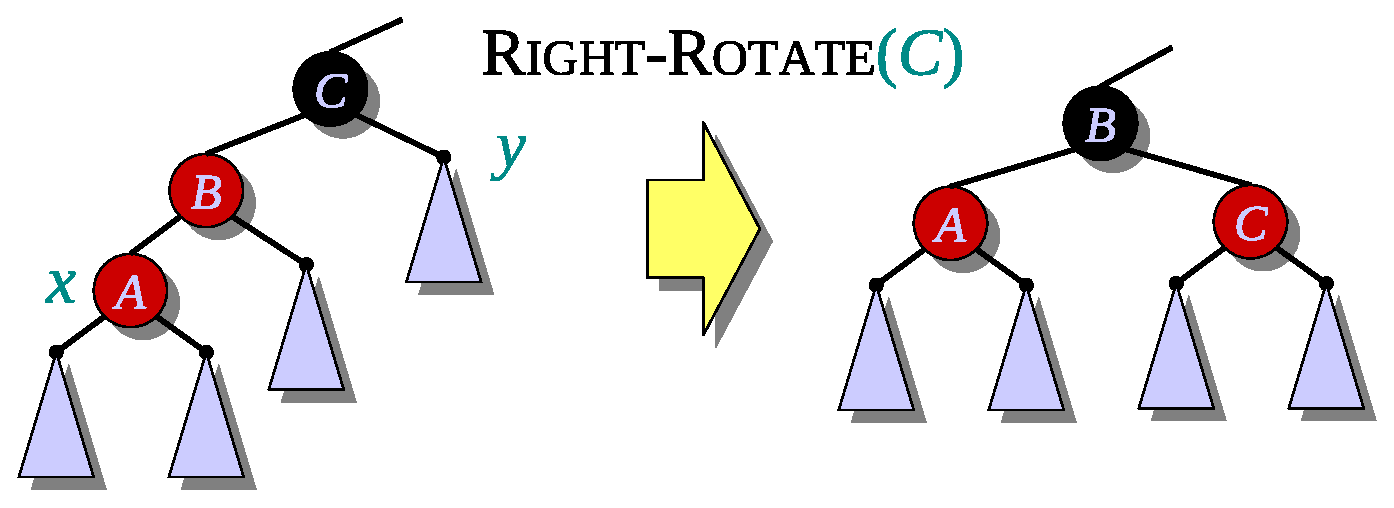
\includegraphics[width=4.5in]{lecture10/case3.eps}
  \caption{Случай 3}
  \label{fig:case3}
\end{figure}
\end{itemize}

\begin{codebox}
\Procname{$\proc{RB\_Insert}(T, x)$}
\li $Tree\_Insert(T, x)$
\li $color[X] \gets RED$
\li \While $x \neq root[T]$ and $color[x] = RED$ \Comment Родитель -- красный
\li   \Do \If $parent[x] = left[parent[parent[x]]]$
\li       \Then $y \gets right[parent[parent[x]]]$ \Comment $y \gets $ ``дядя''
\li           \If $color[y] = RED$ \Comment Можно менять цвет
\li           \Then ... \Comment <Случай 1>
\li           \Else \If $x = right[parent[x]]$
\li                 \Then ... \Comment <Случай 2>
                    \End
\li                 ... \Comment <Случай 3>
              \End
\li       \Else ... \Comment Симметрично, рассматриваем $left$ вместо $right$
          \End
      \End
\li $color[root[T]] \gets BLACK$
\end{codebox}

Крис Окасаки~\cite{Okasaki} предложил альтернативную реализацию красно-чёрных деревьев в функциональной парадигме. В отличии от императивного подхода, имея в распоряжении алгебраические типы данных и механизм pattern matching, можно рассмотреть всего четыре случая, требующие модификации дерева.
\begin{figure}[tp]
  \centering
  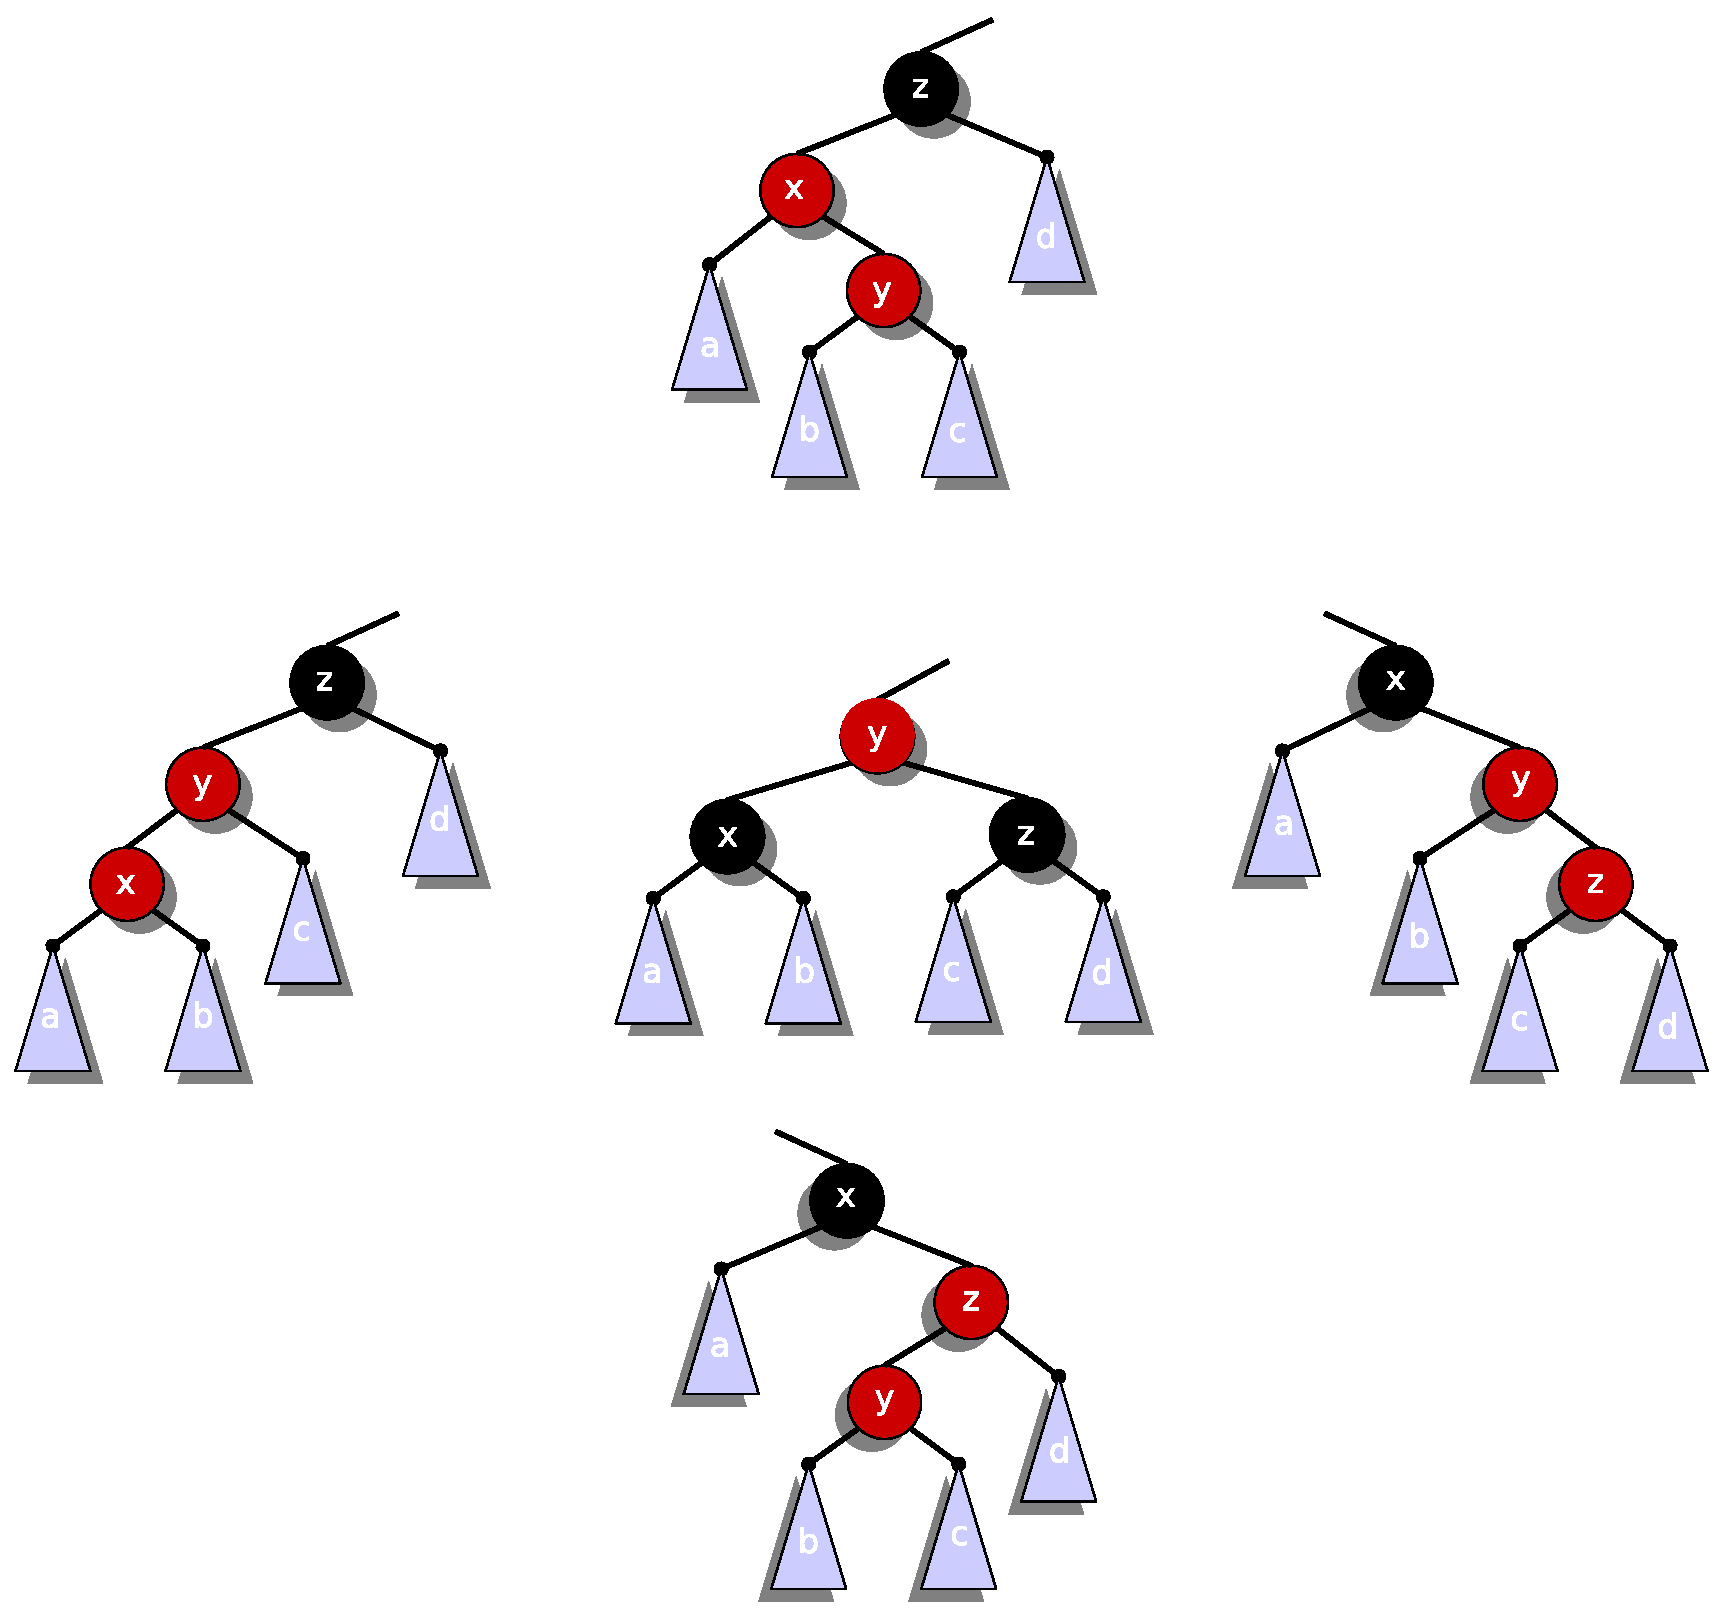
\includegraphics[width=5in]{lecture10/okasaki.eps}
  \caption{Алгоритм Окасаки}
  \label{fig:okasaki}
\end{figure}

Алгоритм Окасаки на Haskell:
\begin{haskell*}
  data Color &=& R | B\\
  data Tree elt &=& E | T Color (Tree elt) elt (Tree elt)\\
  type Set a &=& Tree a\\
  empty &::& Set el\\
  empty &=& E\\
  member &::& Ord elt \Rightarrow elt \to Set elt \to Bool\\
  member x E &=& False\\
  member x (T \_ a y b) &\mid& x < y = member x a\\
  &\mid& x == y = True\\
  &\mid& x > y = member x b\\
  insert &::& Ord elt \Rightarrow elt \to Set elt \to Set elt\\
  insert x s &=& makeBlack (ins s)
  \hswhere{%
    ins E &= T R E x E\\
    ins (T color a y b) &\mid x < y &= balance color (ins a) y b\\
    &\mid x == y &= T color a y b\\
    &\mid x > y &= balance color a y (ins b)\\
    makeBlack (T \_ a y b) &= T B a y b\\
    }
  balance B (T R (T R a x b) y c) z d &=& T R (T B a x b) y (T B c z d)\\
  balance B (T R a x (T R b y c)) z d &=& T R (T B a x b) y (T B c z d)\\
  balance B a x (T R (T R b y c) z d) &=& T R (T B a x b) y (T B c z d)\\
  balance B a x (T R b y (T R c z d)) &=& T R (T B a x b) y (T B c z d)\\
  balance color a x b &=& T color a x 
\end{haskell*}

Альтернативная реализация функции balance рассматривает те же случаи, что и в императивном алгоритме:
\begin{haskell*}
  balance B (T R a (T R \_ \_ \_) x b) y (T R c z d) \\
  \mid B (T R a x b (T R \_ \_ \_)) y (T R c z d) \\
  \mid B (T R a x b) y (T R c (T R \_ \_ \_) z d) \\
  \mid B (T R a x b) y (T R c z d (T R \_ \_ \_)) &=& T R (T B a x b) y (T B c z d) \\ 
  \hscom{color flip}
  balance B (T R a (T R \_ \_ \_) x b) y c &=& T B a x (T R b y c) \\
  balance B a x (T R b y c (T R \_ \_ \_)) &=& T B (T R a x b) y c \\
  \hscom{single rotation} \\
  balance B (T R a x (T R b y c)) z d \\
  \mid B a x (T R (T R b y c) z d) &=& T B (T R a x b) y (T R c z d)\\
  \hscom{double rotation} \\
  balance color a x b &=& T color a x b
\end{haskell*}

Разница между реализациями в количестве выполняемых операций. Например, смена цвета в императивном алгоритме выполняется в три присваивания, а соответствующая трансформация в функциональном -- за семь или больше операций с цветом и с указателями.

Императивный алгоритм выполняет операцию Insert в две фазы: спуск по дереву сверху-вниз со вставкой элемента, затем \emph{балансировка} дерева снизу-вверх. Балансировка может прекратиться до того, как будет достигнут корень дерева.

Функциональный алгоритм выполняет поиск сверху-вниз, а затем \emph{конструкцию} дерева снизу вверх. Процедура конструирования, в отличии от балансировки, не может быть прервана досрочно.

\section{Заключительные замечания}
Одно из основных преимуществ красно-чёрных деревьев заключается в том, что процедуру балансировки практически всегда можно выполнять параллельно с процедурами поиска, т.к. алгоритм поиска не зависит от аттрибута цвета узлов. Вращение поддеревьев не может выполнятся одновременно с поиском, но при вставке выполняется не более $O(1)$ вращений.

Красно-чёрные деревья являются наиболее активно используемыми на практике самобалансирующимися деревьями поиска. В частности, ассоциативные контейнеры библиотеки STL (map, set, multiset, multimap) основаны на красно-чёрных деревьях.

Легко видеть, что красно-чёрные деревья изометричны 2-3-4 B-деревьям. Каждый чёрный узел можно объединить с его красными потомками. Результирующий узел будет иметь не более трех ключей и не более четырех потомков.

\bibliographystyle{alpha}
\bibliography{lecture10}

\end{document}
